\documentclass[11pt]{article}
\usepackage[margin=1in]{geometry}
\usepackage{enumitem}
\usepackage{hyperref}
\usepackage{graphicx}
\usepackage{array}
\usepackage{multicol}
\usepackage{longtable}
\usepackage{titlesec}
\usepackage{float}

\begin{document}

%==================================================
\begin{center}
    \large \textbf{Sri Sivasubramaniya Nadar College of Engineering, Chennai} \\
    (An autonomous Institution affiliated to Anna University) \\
    \vspace{0.3cm}
\end{center}

\begin{table}[!h]
\renewcommand{\arraystretch}{1.5}
\resizebox{\textwidth}{!}{%
\begin{tabular}{|l|cll|}
\hline
Degree \& Branch & \multicolumn{1}{c|}{B.E. Computer Science \& Engineering} & Semester & VI \\ \hline
Subject Code \& Name & \multicolumn{3}{c|}{UCS2612 -- Machine Learning Algorithms Laboratory} \\ \hline
Academic Year & \multicolumn{1}{c|}{2025--2026 (Even)} & Batch & 2023--2027 \\ \hline
Name & Mehanth T & Register No. & 3122235001080 \\ \hline
Due Date & \multicolumn{3}{c|}{27 January 2026} \\ \hline
\end{tabular}
}
\end{table}

\begin{center}
\textbf{Experiment 2: Binary Classification using Na\"ive Bayes and K-Nearest Neighbors}
\end{center}

%==================================================
\section*{1. Aim and Objective}
To implement Na\"ive Bayes and K-Nearest Neighbors (KNN) classifiers for a binary classification problem, evaluate them using multiple performance metrics, visualize model behavior, and analyze overfitting, underfitting, and bias--variance characteristics.

%==================================================
\section*{2. Dataset Description}
A benchmark binary classification dataset containing numerical features and two class labels is used.

Dataset reference:
\begin{itemize}
    \item Kaggle: \href{https://www.kaggle.com/datasets/somesh24/spambase}{Spambase Dataset}
\end{itemize}

The dataset used is the Spambase dataset from the UCI Machine Learning Repository. It consists of 4601 instances, where each instance represents an email. There are 57 continuous real-valued attributes describing the frequency of various words and characters in the email. The target variable is binary: 1 for spam and 0 for non-spam. The dataset is slightly imbalanced, with approximately 39.4\% spam and 60.6\% non-spam emails.

%==================================================
\section*{3. Preprocessing Steps}
The preprocessing steps involved:
\begin{enumerate}
    \item \textbf{Missing Value Check}: The dataset was checked for missing values, and none were found.
    \item \textbf{Data Splitting}: The dataset was split into training (70\%) and testing (30\%) sets using stratified sampling to maintain class distribution.
    \item \textbf{Feature Scaling}:
    \begin{itemize}
        \item \textbf{Min-Max Scaling}: Applied for Multinomial Na\"ive Bayes as it requires non-negative features. Ranges features to [0, 1].
        \item \textbf{Standard Scaling}: Applied for Gaussian Na\"ive Bayes and KNN to standardize features (mean=0, variance=1), which is crucial for distance-based algorithms like KNN.
    \end{itemize}
\end{enumerate}

%==================================================
\section*{4. Implementation Details}
Three variants of Na\"ive Bayes (Gaussian, Multinomial, Bernoulli) were implemented using Scikit-learn. For K-Nearest Neighbors (KNN), the model was tuned to find the optimal number of neighbors ($k$). \n\nHyperparameter tuning strategies:
\begin{itemize}
    \item \textbf{Grid Search}: Exhaustively searched for the best $k$ in range [1, 30] and evaluated weighting schemes ('uniform' vs 'distance').
    \item \textbf{Randomized Search}: Sampled a subset of the parameter space to find optimal settings efficiently.
\end{itemize}
Both KDTree and BallTree algorithms were evaluated for neighbor search efficiency.

%==================================================
\section*{5. Visualizations}

\subsection*{5.1 Exploratory Data Analysis}

\begin{figure}[H]
\centering
\includegraphics[width=0.7\textwidth]{plots/png/class_distribution.png}
\caption{Class Distribution}
\end{figure}

\begin{figure}[H]
\centering
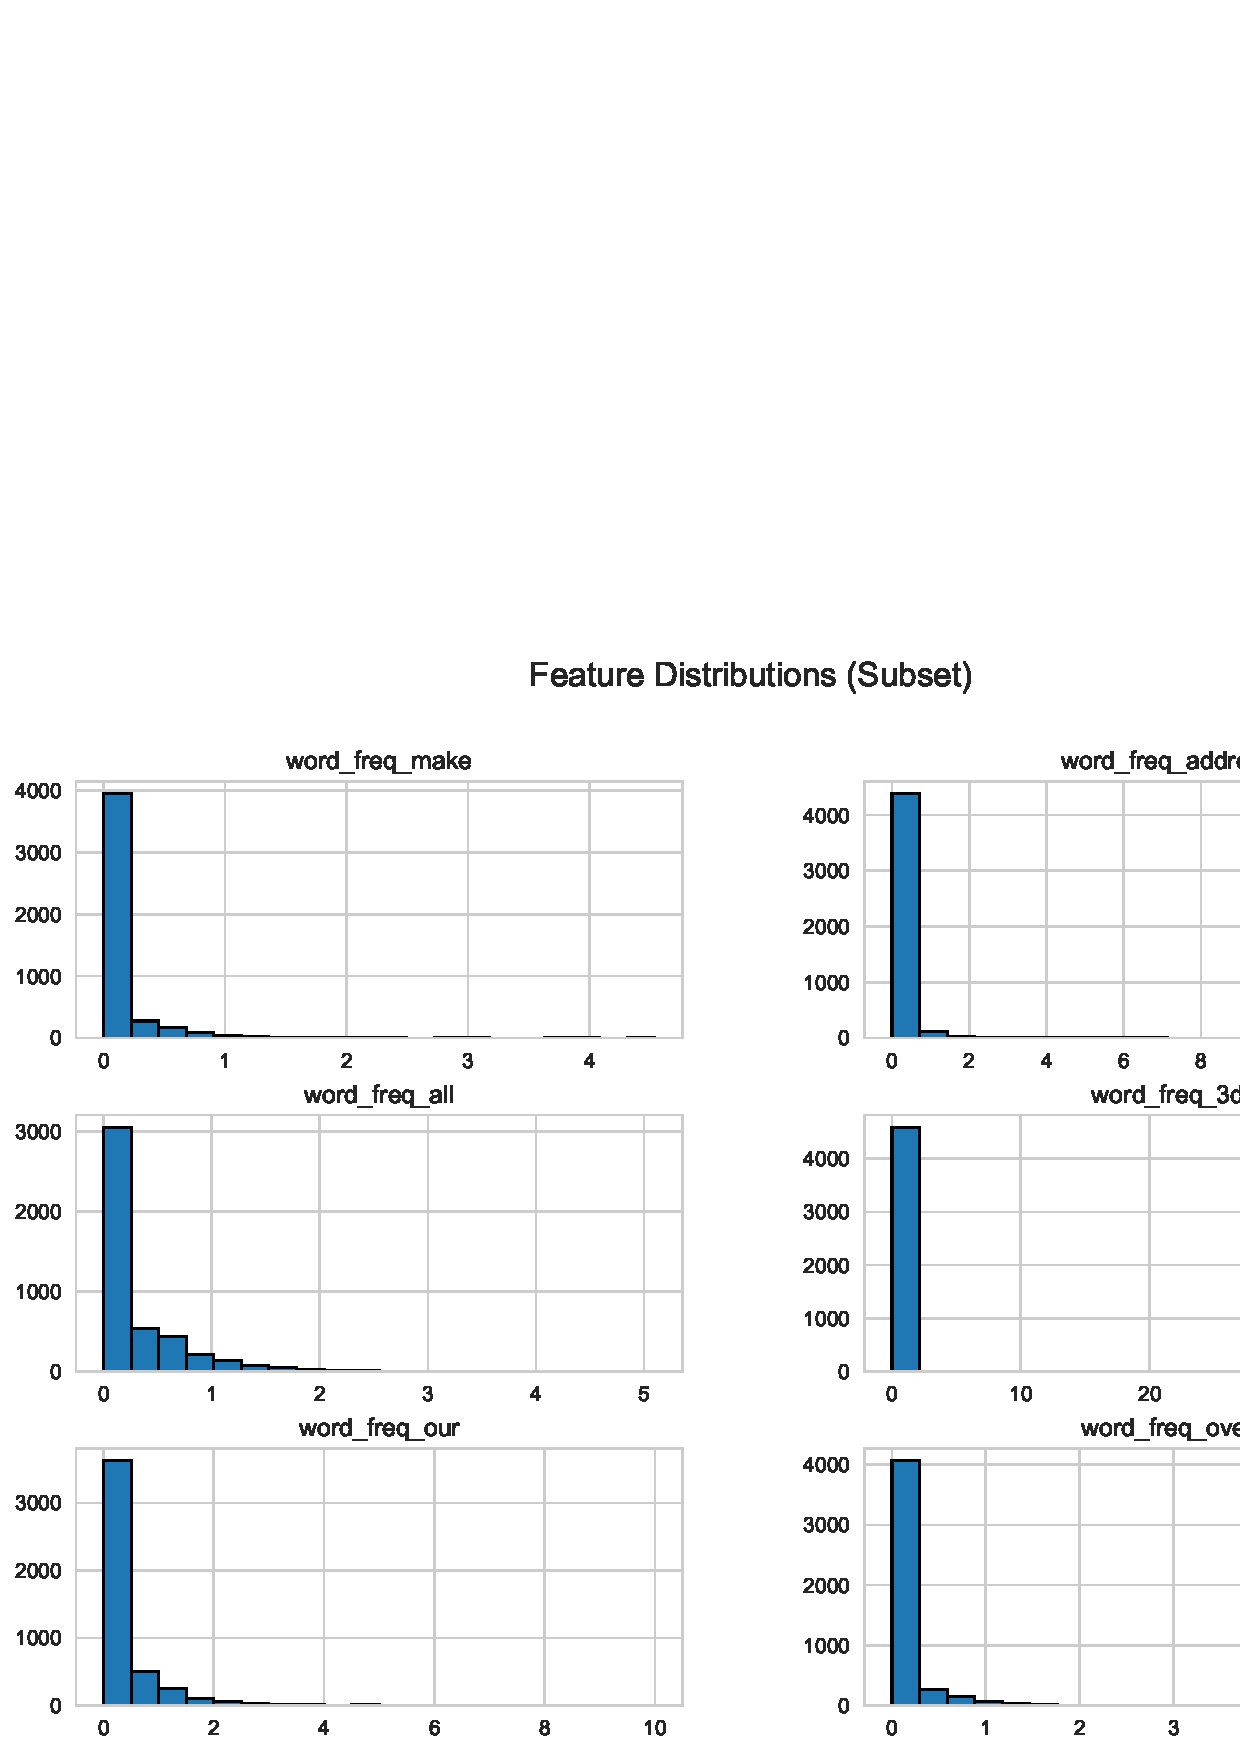
\includegraphics[width=0.9\textwidth]{plots/png/feature_distribution.png}
\caption{Feature Distributions}
\end{figure}

\subsection*{5.2 Model Evaluation}

\begin{figure}[H]
\centering
\includegraphics[width=0.9\textwidth]{plots/png/confusion_matrices.png}
\caption{Confusion Matrices for Classifiers}
\end{figure}

\begin{figure}[H]
\centering
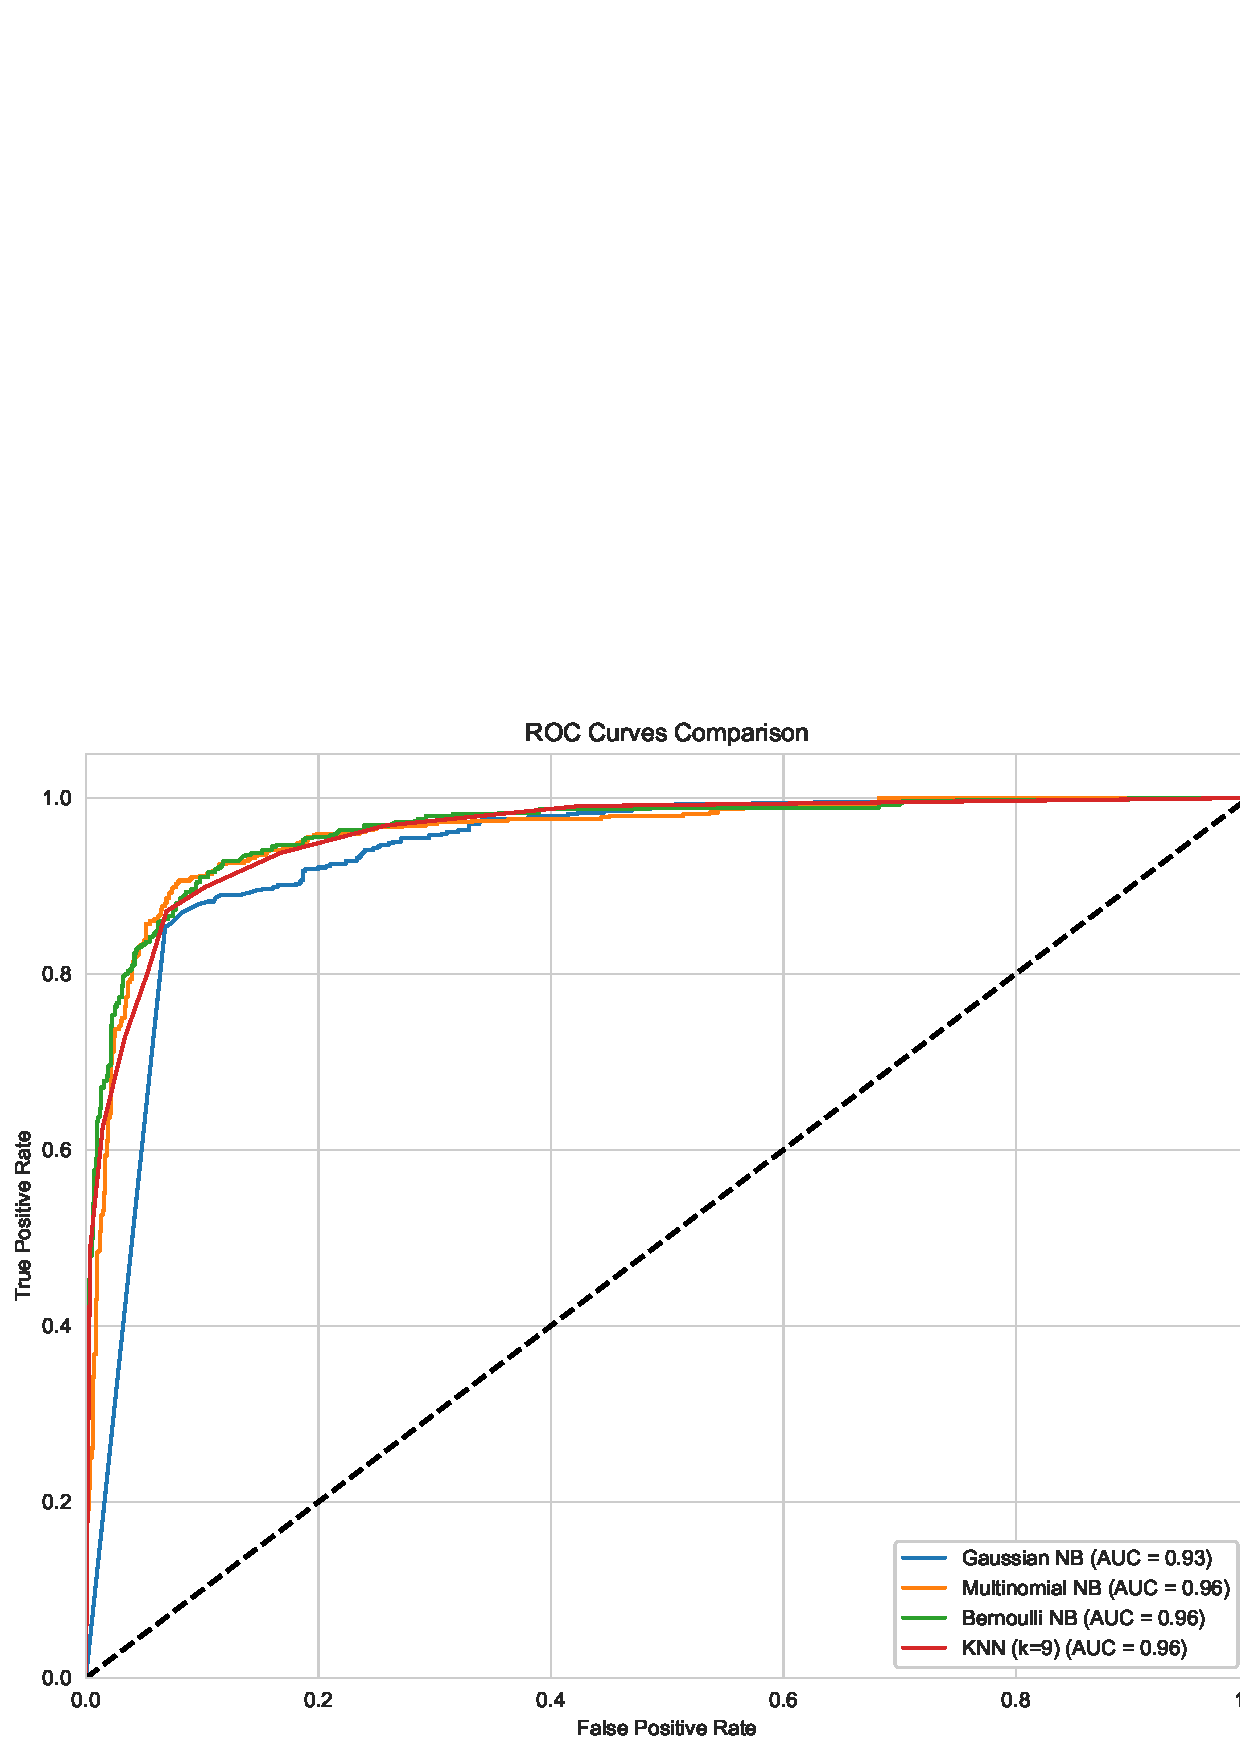
\includegraphics[width=0.8\textwidth]{plots/png/roc_curves.png}
\caption{ROC Curves Comparison}
\end{figure}

\begin{figure}[H]
\centering
\includegraphics[width=0.8\textwidth]{plots/png/knn_accuracy_vs_k.png}
\caption{KNN Accuracy vs k}
\end{figure}

\subsection*{5.3 Bias-Variance Analysis}

\begin{figure}[H]
\centering
\includegraphics[width=0.8\textwidth]{plots/png/learning_curve_nb.png}
\caption{Learning Curve - Naive Bayes}
\end{figure}

\begin{figure}[H]
\centering
\includegraphics[width=0.8\textwidth]{plots/png/learning_curve_knn.png}
\caption{Learning Curve - KNN}
\end{figure}

%==================================================
\section*{6. Performance Tables}

\subsection*{Na\"ive Bayes Performance Comparison}
\begin{table}[H]
\centering
\renewcommand{\arraystretch}{1.3}
\caption{Na\"ive Bayes Performance Metrics}
\begin{tabular}{|l|c|c|c|}
\hline
Metric & Gaussian NB & Multinomial NB & Bernoulli NB \\
\hline
Accuracy & 0.8197 & 0.8965 & 0.9030 \\
Precision & 0.7001 & 0.9293 & 0.9100 \\
Recall & 0.9485 & 0.7978 & 0.8364 \\
F1 Score & 0.8056 & 0.8586 & 0.8716 \\
Specificity & 0.7360 & 0.9606 & 0.9462 \\
Training Time (s) & 0.0033 & 0.0016 & 0.0058 \\
\hline
\end{tabular}
\end{table}

\subsection*{KNN Hyperparameter Tuning Results}
\begin{table}[H]
\centering
\renewcommand{\arraystretch}{1.3}
\caption{KNN Hyperparameter Tuning}
\begin{tabular}{|c|c|c|c|}
\hline
Search Method & Best $k$ & Best CV Accuracy & Best Parameters \\
\hline
Grid Search & 9 & 0.9180 & \{'n\_neighbors': 9, 'weights': 'distance'\} \\
Randomized Search & 9 & 0.9180 & \{'n\_neighbors': 9, 'weights': 'distance'\} \\
\hline
\end{tabular}
\end{table}

\subsection*{KNN Performance using Different Search Methods}

\begin{table}[H]
\centering
\renewcommand{\arraystretch}{1.3}
\caption{KNN Performance using KDTree}
\begin{tabular}{|l|c|}
\hline
Metric & Value \\
\hline
Optimal $k$ & 9 \\
Accuracy & 0.9180 \\
Precision & 0.9010 \\
Recall & 0.8842 \\
F1 Score & 0.8925 \\
Training Time (s) & 0.0070 \\
Prediction Time (s) & 0.0268 \\
\hline
\end{tabular}
\end{table}

\begin{table}[H]
\centering
\renewcommand{\arraystretch}{1.3}
\caption{KNN Performance using BallTree}
\begin{tabular}{|l|c|}
\hline
Metric & Value \\
\hline
Optimal $k$ & 9 \\
Accuracy & 0.9180 \\
Precision & 0.9010 \\
Recall & 0.8842 \\
F1 Score & 0.8925 \\
Training Time (s) & 0.0054 \\
Prediction Time (s) & 0.0388 \\
\hline
\end{tabular}
\end{table}

\subsection*{KDTree vs BallTree Comparison}
\begin{table}[H]
\centering
\renewcommand{\arraystretch}{1.3}
\caption{Comparison of Neighbor Search Algorithms}
\begin{tabular}{|l|c|c|}
\hline
Criterion & KDTree & BallTree \\
\hline
Accuracy & 0.9180 & 0.9180 \\
Training Time (s) & 0.0070 & 0.0054 \\
Prediction Time (s) & 0.0268 & 0.0388 \\
Memory Usage & Low / Medium & Medium / High \\
\hline
\end{tabular}
\end{table}

%==================================================
\section*{7. Overfitting and Underfitting Analysis}
The learning curves indicate that KNN with optimal $k$ and distance weighting achieves better generalization than Gaussian Na\"ive Bayes. As $k$ increases, the model becomes simpler (higher bias), while low $k$ leads to complex boundaries (high variance). The optimal $k=9$ provides a balance. The small gap between training and validation scores in the learning curve suggests the model is not significantly overfitting.

%==================================================
\section*{8. Bias--Variance Analysis}
Na\"ive Bayes (especially Gaussian) typically exhibits higher bias due to its strong independence assumptions, which may not fully hold for word frequencies. However, it requires less training data to converge. KNN is a non-parametric method and typically has lower bias but higher variance (slower convergence of training/validation scores). Hyperparameter tuning helped reduce variance in KNN by selecting an appropriate neighborhood size.

%==================================================
\section*{9. Observations and Conclusion}
In this experiment, KNN ($k=9$) outperformed all Na\"ive Bayes variants in terms of accuracy (91.8\%). Among Na\"ive Bayes models, the Bernoulli and Multinomial variants performed significantly better than Gaussian NB, likely because the word frequency features are better modeled by discrete distributions (after discretization or normalization) than by normal distributions. While KNN offered the best performance, Na\"ive Bayes was extremely fast in both training and prediction, highlighting the trade-off between accuracy and computational efficiency. KDTree provided faster inference than BallTree for this dataset dimensionality.

%==================================================
\section*{References}
\begin{itemize}
    \item \href{https://scikit-learn.org/stable/modules/naive_bayes.html}{Scikit-learn: Na\"ive Bayes}
    \item \href{https://scikit-learn.org/stable/modules/neighbors.html}{Scikit-learn: KNN}
    \item \href{https://scikit-learn.org/stable/modules/grid_search.html}{Scikit-learn: Hyperparameter Optimization}
    \item \href{https://www.kaggle.com/datasets/somesh24/spambase}{Spambase Dataset}
\end{itemize}

\end{document}
